\documentclass [9 pt]{article}
\usepackage[margin = 1in]{geometry}
\usepackage{amsfonts}
\usepackage{amsthm}
\usepackage{bbm}
 \usepackage{amsmath}
\usepackage[utf8]{inputenc}
\usepackage{graphicx}
\usepackage{fancybox}
\usepackage{ wasysym }
\usepackage{enumerate}
\usepackage{color}
\usepackage{graphicx}
\graphicspath{ {./images/} }
\usepackage{tikz}
\usepackage{booktabs}

\theoremstyle{definition}
\newtheorem{problem}{Problem}
\newtheorem{theorem}{Theorem}
\newtheorem*{corollary}{Corollary}
\newtheorem{proposition}[theorem]{Proposition}
\newtheorem{lemma}[theorem]{Lemma}
\newtheorem{conjecture}[theorem]{Conjecture}

\newtheorem{definition}[theorem]{Definition}
\newtheorem{remark}[theorem]{Remark}
\newtheorem{example}[theorem]{Example}


\usepackage{fancyhdr}
\pagestyle{fancy}
\lhead{Yuhao Wu \quad 260711365} 
\rhead{\bfseries COMP 330 Assignment 4}
\cfoot{\thepage}
\renewcommand{\headrulewidth}{0.4pt}
\renewcommand{\footrulewidth}{0.4pt}



\setlength{\parindent}{0pt}

\begin{document}

\title{COMP 330 Assignment 4}
\date{2018-10-25}
\author{Name: Yuhao Wu\\
ID Number: 260711365
}
\maketitle

\section*{Question 1:}
A sequence of parentheses is a sequence of $($ and $)$ symbols or the empty sequence.\\
 Such a sequence is said to be balanced if it has an equal number of $($ and $)$ symbols and in every prefix of the sequence the number of left parentheses is greater than or equal to the number of right parentheses. Thus $((())())$ is balanced but, for example, $())($ is not balanced even though there are an equal number of left and right parentheses. The empty sequence is considered to be balanced.
 Consider the grammar
$$S \to (S)\ |\ SS\ |\ \varepsilon$$
This grammar is claimed to generate balanced parentheses.
\begin{itemize}
	\item Prove that any string generated by this grammar is a properly balanced sequence of parentheses.
	\item Prove that every sequence of balanced parentheses can be generated by this grammar.
\end{itemize}

\newpage
\subsection*{(a):}
We will show "any string generated by this grammar is a properly balanced sequence of parentheses" by induction on the number of derivation steps.
\begin{itemize}
	\item \textbf{Base Case:} \\
	If the derivation has only one step then the derivation must be $S\to \varepsilon $, obviously, we have $\varepsilon$ is a properly balanced sequence of parentheses.
	\item \textbf{Inductive Step:}\\
	We assume for $w$, after $n \ (n \leq k)$ derivations, we will get a properly balanced sequence of parentheses.\\\\
	So, we now consider an $(n + 1)$ step derivation of $w$, it has two forms:
	\begin{itemize}
		\item[1] $S \to (S) \xrightarrow{*} (x) = w \quad $ in this case, $S \xrightarrow{*} x$ is less than or equal to $k$ derivations. So, we have $x$ as a balanced sequence of parentheses.\\\\
		Obviously, $(x)$ has an equal number of right parenthesis and left parenthesis. \\
		Since the left parenthesis is added in the front of $x$ and for $x$ and every prefix of $S$,  for every prefix of $(x)$, the number of left parenthesis is also greater than or equal to that of right parenthesis.\\
 		 \bigg(the equal happens when the prefix is the whole word $(x)$\bigg)\\
  		\\
  		\\
  		\item[2] $S \to SS \xrightarrow{*} x_1x_2 = w \quad $ in this case, $S \xrightarrow{*} x_1$ is less than or equal to $k$ derivations. So is $S \xrightarrow{*} x_2$. we have $x_1, x_2$ as a balanced sequence of parentheses.\\\\
  		Since $x_1, x_2$ has an equal number of right and left parenthesis, $w = x_1x_2$ also has an equal number of right and left parenthesis.\\
  		\\
  		$w = x_1x_2$, if we look from left to right until $x_1$, according $x_1$ is properly balance string, we know for this part, every prefix the number of left parenthesis is greater than or equal to that of right parenthesis.\\
  		Now we consider the case prefix of $w$ is of the form $x_1x_2'$ where  $x_2'$ is the prefix of $x_2$. For every prefix of $x_2$ we have $\#( \ \geq \# )$, and $x_1$ has equal number of left parenthesis and right parenthesis. So, for every prefix of $w = x_1x_2$, we still have $\#( \ \geq \# )$ \\
	\end{itemize}
	 So, $w$ is a properly balanced sequence of parentheses.
\end{itemize}
Now, we can say any string any string generated by this grammar has [1] equal number of left parenthesis and right parenthesis and [2] in every prefix of the sequence the number of left parentheses is greater than or equal to the number of right parentheses, which is a properly balanced sequence of parentheses






















\newpage

\subsection*{(b):}
We now need to prove that every sequence of balanced parentheses can be generated by this grammar.\\
\\
Let $w$ be the string of balanced parentheses. We can use induction on the length of $w$ to show $w$ can be generated by the given grammar.\\
\\
\textbf{Base Case:} Suppose that $w = \varepsilon$. Since the grammar has rule $B \to \varepsilon$, we can see it generates $w$.\\
\\
\\
\textbf{Induction Step:} \\\\
\textbf{Induction Hypothesis:}
Suppose that every sequence of balanced parentheses whose length is less than $n$ can be generated by this grammar.
\\
\\
Now we assume $|w| = n$, and consider the least $k > 1$ such that the prefix of $w$ of length $k$ has the same number of $($ as $)$.
\begin{itemize}
	\item If $k = n$, then we write $w$ as $w = (w_1)$, now we need to show $w_1$ is a string of balanced parentheses.
	\begin{itemize}
		\item As there are same number $($ as $)$ in $w = (w_1)$, so, for $w_1$, there are same number of  $($ and $)$ as well.
		\item Suppose that some prefix of $w_1$ has more $)$ than $($, then there exists some $w_1'$ has exactly one more $)$ than $($, so k is not the least, as the prefix $(w_1'$ has the same number of ('s and )'s and has length less than $k$. So, for every prefix of $w_1$, $\#(\ \geq \ \#)$
	\end{itemize}
	So, we can now say $w_1$ is a string of balanced parentheses.\\
	According to our hypothesis, we can say $w_1$ can be generated by CFG.\\
	Using the rule $ S \to (S) $, $w = (w_1)$ can also be generated by CTG\\
	\\
	\item If $k < n$, then we write $w$ as $w = (w_1)w_2$, where $|(w_1)| = k$ now we need to show $w_1, w_2$ is a string of balanced parentheses.
	\begin{itemize}
		\item according to previous case, we have $w_1$ has the same number of ( and ), and for every prefix of $w_1$, $\#(\ \geq \ \#)$, which means $w_1$ is a string of balanced parentheses.
		\item As there are as manny ('s and )'s in both $w$ and $(w_1)$, it is the same in $w_2$
		\item For every prefix $w_2'$ of $w_2$,  $(w_1)w_2'$ is also a prefix of $w$, as we know for every prefix of $w$, $\#(\  \geq \ \#)$ and for $(w_1)$, the number of ( is the same as ), so for every prefix $w_2'$ of $w_2$, we still have $\#(\  \geq \ \#)$
	\end{itemize}
	So, we can conclude that $w_1, w_2$ is a string of balanced parentheses.
	According to our hypothesis, we can say $w_1, w_2$ can be generated by CFG.\\
	Using the rule $ S \to (S) $, $(w_1)$ can also be generated by CTG\\
	Using the rule $ S \to SS $, $w = (w_1)w_2 $ can also be generated by CTG\\

\end{itemize}
Thus, we can conclude that  every sequence of balanced parentheses can be generated by this grammar.\\




\newpage
\section*{Question 2:}
 Consider the following context-free grammar:
 $$S \to aS\ |\ aSbS \ |\  \varepsilon$$
 
This grammar generates all strings where in every prefix the number of a’s is greater than or equal to the number of b’s. Show that this grammar is ambiguous by giving an example of a string and showing that it has two different derivations.
\\
\\
\\
\textbf{ I choose string $aab$ }\\
\begin{center}
\begin{tikzpicture}
  \node(0){$S$}
     child{node{$a$}}
     child{node{$S$}
       child{node{$a$}}
       child{node{$S$}
       	child{node{$\varepsilon$}}}
       child{node{$b$}}
       child{node{$S$}
       child{node{$\varepsilon$}}}
     };
\end{tikzpicture}
\end{center}

\begin{center}
\begin{tikzpicture}
  \node(0){$S$}
     child{node{$a$}}
     child{node{$S$}
     	 child{node{$a$}}
     	  child{node{$S$} 
     	    child{node{$\varepsilon$}}}   }
     child{node{$b$}}
     child{node{$S$}
       child{node{$\varepsilon$}}
     };
\end{tikzpicture}
\end{center}












\newpage
\section*{Question 3: }
We define the language $PAREN_2$ inductively as follows:
\begin{itemize}
	\item  $ \varepsilon \in PAREN_2$
	\item if $x \in PAREN_2$ then so are $(x)$ and $[x]$
	\item  if $x$ and $y$ are both in $PAREN_2$ then so is $xy$.
\end{itemize}
Describe a PDA for this language which accepts by empty stack. Give all the transitions.\\
\\\\
\textbf{SOLUTION:}
\begin{center}
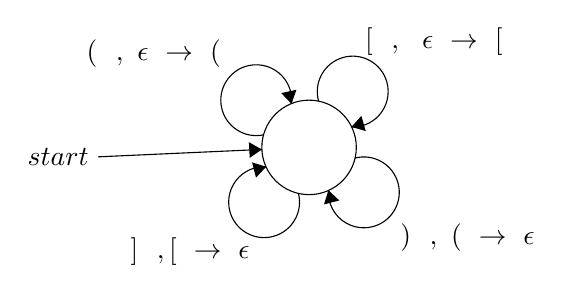
\begin{tikzpicture}[scale=0.2]
\tikzstyle{every node}+=[inner sep=0pt]
\draw [black] (33.3,-22.4) circle (3);
\draw [black] (33.909,-19.474) arc (195.96971:-92.03029:2.25);
\draw (41.22,-16.59) node [above] {$[\ \ ,\mbox{ }\mbox{ }\epsilon\mbox{ }\to \mbox{ }[$};
\fill [black] (35.99,-21.1) -- (36.9,-21.36) -- (36.62,-20.4);
\draw [black] (36.21,-23.078) arc (104.60876:-183.39124:2.25);
\draw (39.07,-28.12) node [right] {$)\ \ ,\mbox{ }(\mbox{ } \to \mbox{ }\epsilon$};
\fill [black] (34.53,-25.12) -- (34.25,-26.02) -- (35.22,-25.77);
\draw [black] (30.421,-21.601) arc (282.21596:-5.78404:2.25);
\draw (27.73,-16.45) node [left] {$( \ \ ,\mbox{ }\epsilon\mbox{ } \to \mbox{ }($};
\fill [black] (32.18,-19.63) -- (32.5,-18.74) -- (31.53,-18.95);
\draw [black] (32.621,-25.31) arc (14.60757:-273.39243:2.25);
\draw (25.75,-28.11) node [below] {$] \ \ ,[\mbox{ }\to \mbox{ }\epsilon$};
\fill [black] (30.58,-23.63) -- (29.68,-23.35) -- (29.93,-24.32);
\draw [black] (19.9,-23) -- (30.3,-22.53);
\draw (19.33,-23.02) node [left] {$start$};
\fill [black] (30.3,-22.53) -- (29.48,-22.07) -- (29.53,-23.07);
\end{tikzpicture}
\end{center}

As this question asks for a PDA for this language which accepts by empty stack, we do not need accept states any more. It will accept the word if there is no input anymore and the stack is empty.\\
\\
It pushes open parentheses and brackets into the stack and pops them off if it sees the matched closed parentheses and brackets.\\
\\
All the other transition which is not on the graph will lead the PDA to jam
\\






\newpage
\section*{Question 4: }
Consider the language $\{a^n\ b^m\ c^p \ |\ n \leq p\ or\ m \leq p\}$.\\
\\
 Show that this is context free by giving a grammar. You need not give a formal proof that your grammar is correct but you must explain, at least briefly, why it works.\\
 \\
 \textbf{SOLUTION:}\\
 To begin with, I will give the grammar first.

 	$$S \to M | AN | SC$$ 
 	$$M \to aMc | B \quad\quad \text{M builds equal numbers of a's and c's}$$
 	$$N \to bNc | \varepsilon \quad\quad \text{N builds equal numbers of b's and c's} $$
 	$$A \to aA | \varepsilon \quad\quad \text{this builds a list of a's}$$
 	$$B \to bB | \varepsilon \quad\quad \text{this builds a list of b's}$$
 	$$C \to cC | \varepsilon \quad\quad \text{this builds a list of c's}$$ 
\\
Then, I will show every world in the language $L = \{a^n\ b^m\ c^p \ |\ n \leq p\ or\ m \leq p\} $ can be generated by the grammar.\\
As we can see, if the world $w \in L$, the number of $c$ must be greater than the number of $a$ or the number of $c$, which means $p > min(n, m)$
\begin{itemize}
	\item Suppose that $n \leq m$, then we can write $w \ as\ w = a^n\ b^m\ c^n\ c^{p-n} $, we write $w = w_1 \cdot w_2 = (a^n\ b^m\ c^n) \cdot c^{p-n} $\\
	Obviously, we can generate $w_1 = a^n\ b^m\ c^n $ using rule $M \to aMc | B$ combined with rule $B \to bB | \varepsilon$.\\
	Then, by rule $S \to M$, we have $w_1$ can be generated by the grammar. \\
	We can generate $w_2 = c^{p-n}$ using rule $C \to cC | \varepsilon$.\\
	Finally, use the rule $S \to SC$, we can get $w = w_1\cdot w_2$ can be generated by the grammar.\\
	\item Suppose that $n > m$, then we can write $w \ as\ w = a^n\ b^m\ c^m\ c^{p-m} $, we write $w = w_1 \cdot w_2 = (a^n\ b^m\ c^m) \cdot c^{p-m} $\\
	Obviously, we can generate $\ b^m\ c^m $ using rule $N \to bNc |\varepsilon $ ,\\
	we can generate $\ a^n $ using rule $A \to aA | \varepsilon$.\\
	Then, by rule $S \to AN$, we have $w_1 = (a^n\ b^m\ c^m) $ can be generated by the grammar. \\
	We can generate $w_2 = c^{p-n}$ using rule $C \to cC | \varepsilon$.\\
	Finally, use the rule $S \to SC$, we can get $w = w_1\cdot w_2$ can be generated by the grammar.\\

	
\end{itemize}
Then, I will show that, every string generated by the grammar is in $L = \{a^n\ b^m\ c^p \ |\ n \leq p\ or\ m \leq p\} $\\\\
As we can see, $M$ generates the same number of a's and c's, so, the rule $S \to M$ always gives $n = p$, if it is combined with rule $S \to SC$, we can have $n \leq P$\\
And, $N$ generates the same number of b's and c's, so, the rule $S \to AN$ always gives $m = p$, if it combines with the rule $S \to SC$, we can have $m \leq P$\\
Thus, we can say that every string generated by the grammar is in $L = \{a^n\ b^m\ c^p \ |\ n \leq p\ or\ m \leq p\} $





















 \newpage
 \section*{Question 5:}
 A linear grammar is one in which every rule has exactly one terminal and one non-terminal on the right hand side or just a single terminal on the right hand side or the empty string. Here is an example
 $$S \to aS\ |\ a\ |\ bB;\quad\quad B \to bB\ |\ b.$$
 \begin{itemize}
 	\item Prove that any regular language can be generated by a linear grammar. I will be happy if you show me how to construct a grammar from a DFA; if your construction is clear enough you can skip the straightforward proof that the language generated by the grammar and the language recognized by the DFA are the same.
 	\item Is every language generated by a linear grammar regular? If your answer is “yes” you must give a proof. If your answer is “no” you must give an example.

 \end{itemize}
 
 
\subsection*{(a):}
\begin{itemize}
	\item To begin with, we use all the \textbf{alphabet of the DFA} as the \textbf{Terminal of our CFG}:\\
	\item Then, we use all the \textbf{states of the DFA} as the \textbf{non-Terminal of CFG}:\\
	\item Then we need to choose a start symbol $S \in V$, the \textbf{start symbol} is the same as the \textbf{start state in DFA}:\\
	\item Now, for each non-Terminal (each states of the DFA), we have a transition function in this form $\delta(S_i, a) = S_j$, then we can convert the transition function into CFG rules $S_i \to aS_j$:\\
	\item Now, we need to end our grammar. For those $\delta(S_i, a) = S_j$, \\
	if $S_j$ is the accept state, we need to add one more rule $S_j \to \varepsilon$\\
	if the start state $S_0$ is also accept state, we need to add $S_0 \to \varepsilon $
\end{itemize}

\newpage
I used a concrete DFA to make my way to construct the grammar more clear.
\begin{center}
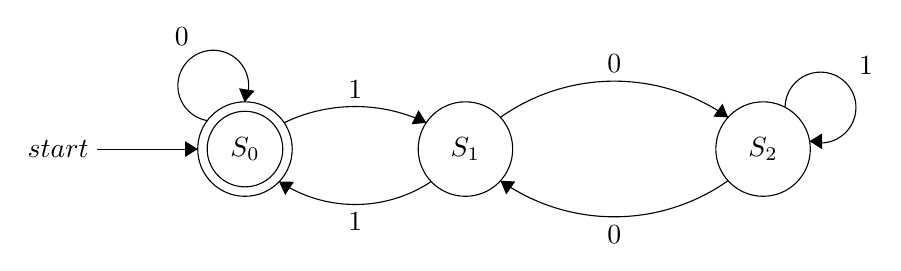
\begin{tikzpicture}[scale=0.2]
\tikzstyle{every node}+=[inner sep=0pt]
\draw [black] (22.5,-26.2) circle (3);
\draw (22.5,-26.2) node {$S_0$};
\draw [black] (22.5,-26.2) circle (2.4);
\draw [black] (36.5,-26.2) circle (3);
\draw (36.5,-26.2) node {$S_1$};
\draw [black] (55.4,-26.2) circle (3);
\draw (55.4,-26.2) node {$S_2$};
\draw [black] (13.1,-26.2) -- (19.5,-26.2);
\draw (12.6,-26.2) node [left] {$start$};
\fill [black] (19.5,-26.2) -- (18.7,-25.7) -- (18.7,-26.7);
\draw [black] (24.98,-24.53) arc (115.70449:64.29551:10.421);
\fill [black] (34.02,-24.53) -- (33.52,-23.73) -- (33.08,-24.63);
\draw (29.5,-23) node [above] {$1$};
\draw [black] (34.336,-28.257) arc (-56.31311:-123.68689:8.719);
\fill [black] (24.66,-28.26) -- (25.05,-29.12) -- (25.61,-28.28);
\draw (29.5,-30.22) node [below] {$1$};
\draw [black] (38.718,-24.19) arc (125.31606:54.68394:12.511);
\fill [black] (53.18,-24.19) -- (52.82,-23.32) -- (52.24,-24.14);
\draw (45.95,-21.39) node [above] {$0$};
\draw [black] (53.179,-28.206) arc (-54.76026:-125.23974:12.529);
\fill [black] (38.72,-28.21) -- (39.09,-29.08) -- (39.66,-28.26);
\draw (45.95,-31) node [below] {$0$};
\draw [black] (20.119,-24.395) arc (260.56505:-27.43495:2.25);
\draw (18.49,-19.66) node [above] {$0$};
\fill [black] (22.48,-23.21) -- (23.11,-22.5) -- (22.12,-22.34);
\draw [black] (56.798,-23.559) arc (179.83765:-108.16235:2.25);
\draw (61.46,-20.87) node [right] {$1$};
\fill [black] (58.35,-25.7) -- (59.15,-26.21) -- (59.15,-25.21);
\end{tikzpicture}
\end{center}
\begin{itemize}
	\item To begin with, we use all the \textbf{alphabet of the DFA} as the \textbf{Terminal of our CFG}:\\
	so, the terminal is $T = \{ 0, 1 \}$
	\item Then, we use all the \textbf{states of the DFA} as the \textbf{non-Terminal of CFG}:\\
	$V = \{ S_0, S_1, S_2 \}$
	\item Then we need to choose a start symbol $S \in V$, the \textbf{start symbol} is the same as the \textbf{start state in DFA}:\\
	$S = \{ S_0 \}$
	\item Now, for each non-Terminal (each states of the DFA), we have a transition function in this form $\delta(S_i, a) = S_j$, then we can convert the transition function into CFG rules $S_i \to aS_j$:
	In our case, we have:
	\begin{align*}
		S_0 &\to 0S_0\ |\ 1S_1\\
		S_1 &\to 0S_2\ |\ 1S_0\\
		S_2 &\to 1S_2\ |\ 0S_1\\
	\end{align*}
	\item Now, we need to end our grammar. For those $\delta(S_i, a) = S_j$, \\
	if $S_j$ is the accept state, we need to add one more rule $S_j \to \varepsilon$\\
	if the start state $S_0$ is also accept state, we need to add $S_0 \to \varepsilon $
	\begin{align*}
		S_0 &\to 0S_0\ |\ 1S_1\ |\ \varepsilon \\
		S_1 &\to 0S_2\ |\ 1S_0\\
		S_2 &\to 1S_2\ |\ 0S_1\\
	\end{align*}
\end{itemize} 
 




\subsection*{(b):} 
$$ S \to aA\ |\ \varepsilon$$
$$ A \to Sb  $$
As we can see, this grammar can generate string in the form $a^n\ b^n$, which we know is non-regular.

\end{document}